% MediSense-Cardio -- IEEE conference paper (assembled draft)
% Built 2026-09-24 from docs/PAPER-*-DRAFT.md. Uses the standard IEEEtran conference
% class, available by default on Overleaf (no upload needed there). If compiling
% locally, IEEEtran.cls must be on the TeX path (install via your TeX distribution's
% package manager, e.g. `tlmgr install ieeetran`, or download from
% https://www.ieee.org/conferences/publishing/templates.html).
%
% This file resolves the open [TODO]s from the source drafts as follows, matching the
% honest, unfinished state of the project as of 2026-09-24:
%   - Contribution list states only what has actually been run (Contribution 1,
%     heart-rate tier). Contribution 2 is named as proposed/future work, not delivered.
%   - The blur/resolution mechanism (Section V-A) is stated as a hypothesis, not a
%     confirmed finding, since the digitizer's internals were not instrumented.
%   - NeuroKit2 is cited by name and URL via footnote (verified in docs/REFERENCES.md,
%     Topic 3) rather than as a numbered reference, since no formal citation for it was
%     verified in the existing reference list -- add one before final submission if a
%     numbered citation is required by the venue.
% Everything else is a direct, unmodified assembly of PAPER-METHOD-DRAFT.md,
% PAPER-RESULTS-DRAFT.md, PAPER-INTRO-RELATEDWORK-DRAFT.md,
% PAPER-DISCUSSION-LIMITATIONS-DRAFT.md, and PAPER-ABSTRACT-CONCLUSION-DRAFT.md.
%
% UPDATE 2026-09-25: a second sweep (v2) was run, keeping the digitized signal long
% enough to also measure PR/QRS/QT/QTc via NeuroKit2 delineation, resolving what was
% previously this paper's single largest limitation ("heart rate only"). That
% delineation-based measurement carries its own real baseline noise floor (median
% ~20ms disagreement between ground-truth and digitized delineation on the CLEAN
% image, vs ~0.1bpm for heart rate) -- documented honestly rather than hidden. The
% raw error-magnitude trend across degradation levels is robust and confirms the
% same blur/resolution pattern as heart rate; the QTc threshold-crossing outcome
% (analogous to false reassurance) is reported separately and more cautiously, since
% naive counting was confounded by that baseline noise (32 of 38 apparent events were
% artefacts of records already misclassified on their own clean image -- corrected by
% requiring the same record be classified correctly on its clean image before a
% degraded-level flip counts as real). All local analysis code:
% scripts/analysis/analyze_v2_intervals.py; data: results/v2_intervals/.

\documentclass[conference]{IEEEtran}
\IEEEoverridecommandlockouts
\usepackage{cite}
\usepackage{amsmath,amssymb,amsfonts}
\usepackage{graphicx}
\usepackage{textcomp}
\usepackage{xcolor}
\usepackage{booktabs}
\usepackage{url}

\def\BibTeX{{\rm B\kern-.05em{\sc i\kern-.025em b}\kern-.08em
    T\kern-.1667em\lower.7ex\hbox{E}\kern-.125emX}}

\begin{document}

\title{From Paper to Patient: Quantifying Digitization-Induced False Reassurance in Automated ECG Explanation\\
\large \textit{[Working title -- confirm against docs/PLAN.md before submission]}}

% TODO: fill in author block, affiliations, and emails before submission.
\author{
\IEEEauthorblockN{Author Name(s) [TODO]}
\IEEEauthorblockA{\textit{Department [TODO]} \\
\textit{Institution [TODO]} \\
City, Country [TODO] \\
email@example.com [TODO]}
}

\maketitle

\begin{abstract}
Patients increasingly encounter automated systems that read a photographed paper ECG
and explain it in plain language, but such pipelines are typically validated on
clean, well-scanned images -- not on the blurred, tilted, or low-resolution photos
patients actually take. We study how much image degradation an automated
digitize-and-explain pipeline can tolerate before it gives a patient a falsely
reassuring answer. We build an end-to-end measurement harness -- render, degrade,
digitize, and compare against ground truth -- over a stratified sample of 50 PTB-XL
records, spanning six independent degradation axes (blur, rotation, JPEG compression,
resolution, brightness/shadow, grid contrast) at five severities each plus a clean
baseline (1{,}550 tests total). On clean images, all reliably-digitized records were
read correctly. Under degradation, heart-rate error rose along only two of the six
axes -- blur and low resolution -- and only at their most severe level, where the
system misclassified 2 of 9 and 4 of 9 at-risk records, respectively, as within
normal range when they were not: a real, clinically meaningful false reassurance. The
remaining four axes (rotation, JPEG compression, grid-contrast fade, brightness)
degraded gracefully, at worst producing no reading rather than a wrong one. A further
6 of 50 records were unreliable to digitize regardless of degradation, independent of
image quality. A second measurement pass extracted PR interval, QRS duration, and
QT/QTc from the digitized signal and confirmed the same blur/resolution pattern at
the level of raw error magnitude, on top of a real $\sim$20~ms baseline delineation
noise floor; a QTc-threshold analogue of false reassurance, corrected for that
baseline noise, found a smaller, less concentrated signal (6 events across 19
at-risk records) that we report as exploratory rather than conclusive. These results
indicate that quality-based safeguards for this kind of system need not treat all
degradation uniformly: two specific, identifiable failure conditions account for the
safety-relevant risk observed, and could form the basis of a targeted upload-time
quality check.
\end{abstract}

\begin{IEEEkeywords}
electrocardiogram, ECG digitization, image degradation, patient-facing AI, false
reassurance, medical AI safety, uncertainty
\end{IEEEkeywords}

\section{Introduction}

An ECG (electrocardiogram) taken at a clinic is normally read by trained staff on
calibrated equipment. Increasingly, patients instead encounter a printed or
photographed ECG outside that setting -- a printout from a home device, a photo of a
clinic report sent over a messaging app, an image uploaded to a symptom-checking
service -- and expect a system that can read it back into numbers and explain what
those numbers mean in plain language. Systems of this shape are already technically
feasible: open-source tools can digitize a paper ECG image into a waveform with
reported signal-to-noise around 19.65~dB on real-world scanned pages \cite{ref5}, and
large language models are routinely used to translate structured clinical output
into plain-language text for patients \cite{ref33,ref34,ref38,ref39,ref40,ref41,ref42,ref43}.

What is not established is what happens when the \emph{input image itself} is
degraded -- blurred, tilted, poorly lit, low-resolution, or compressed -- as a
patient's own phone photo very often will be. Each stage of a digitize-then-explain
pipeline is normally validated on clean, well-scanned images. If the extracted heart
rate (or interval) is wrong because the source image was poor, and the pipeline is
confident anyway, the final sentence shown to the patient can be \textbf{false
reassurance}: a system stating that an abnormal reading is normal. This is a
safety-relevant failure specific to the image$\to$numbers$\to$text pipeline as a
whole, not to any one stage of it, and -- as Section~II argues -- it has not been
directly measured.

\subsection{Problem statement and research question}

We ask: \emph{how much does image degradation of a photographed paper ECG have to
accumulate before an automated digitize-and-explain pipeline gives a patient a
factually wrong, falsely reassuring answer?} We answer this empirically rather than
theoretically, using a pipeline built from existing, previously-validated open-source
components (Section~III), a public ECG dataset with known ground truth \cite{ref45},
and a systematic, controlled degradation study spanning six realistic image-quality
axes at five severities each (Section~III-C).

\subsection{Contribution}

This paper's contribution, as currently supported by evidence, is twofold:

\begin{enumerate}
\item We build and run an end-to-end, repeatable degradation-measurement harness --
render (ECG-Image-Kit \cite{ref1}) $\to$ controlled multi-axis degradation $\to$
digitize (Open-ECG-Digitizer \cite{ref5}) $\to$ compare against ground truth -- over a
stratified, labeled sample of PTB-XL records \cite{ref45}, covering six independent
degradation axes (blur, rotation, JPEG compression, resolution, brightness/shadow,
grid contrast) at five severities each.
\item We report, to our knowledge for the first time (Section~II), how digitization
error at this severity range translates into the \emph{patient-facing} outcome that
matters -- not signal-level error alone, but whether the system would tell a patient
with an abnormal heart rate that they are within normal range -- and show that this
happens only at the two most severe levels of two of the six axes tested (blur,
resolution), while the other four axes degrade gracefully into ``no answer'' rather
than a wrong one.
\item We extend the measurement beyond heart rate to PR interval, QRS duration, and
QT/QTc (Section~IV-F), confirming the same blur/resolution error pattern at the
interval level and reporting, with appropriate caution, an analogous QTc-based
false-reassurance signal after correcting for a real baseline delineation-noise
confound we identify and document rather than overlook.
\end{enumerate}

A calibrated no-reference image-quality proxy that would predict these failures
without needing ground truth at inference time is proposed as future work
(Section~VI) but has not yet been built or evaluated, and is therefore not claimed as
a delivered contribution of this paper.

\subsection{Paper organization}

Section~II situates this work against ECG digitization, ECG signal-quality
assessment, uncertainty-aware medical AI, and patient-facing medical text generation.
Section~III describes the dataset, pipeline, and degradation model. Section~IV
reports results. Section~V discusses the findings, Section~VI states limitations, and
Section~VII concludes.

\section{Related Work}

We organize related work around the three fields this project sits between: (A)
digitizing paper ECGs, which we reuse rather than contribute to; (B) assessing
whether a signal or image is good enough to trust, the closest published work to the
first half of our contribution; (C) knowing when an automated system should decline
to answer, the closest published work to the second half; and (D) generating
patient-facing medical text safely, which bounds how novel our end-to-end framing can
honestly be claimed to be.

\subsection{ECG digitization}

Converting a printed or photographed ECG into a digital waveform is an active area
that is mature for clean scans but not yet for phone photographs. ECG-Image-Kit \cite{ref1} provides a synthetic-image
generation toolbox that we use to render controlled test images from ground-truth
PTB-XL signals (Section~III-B). On the reading side, several open digitizers now
report strong accuracy on real scanned pages: Open-ECG-Digitizer \cite{ref5}, which we
use, is validated on 37{,}191 ECG images with reported SNR near 19.65~dB;
ECGtizer \cite{ref3} and ECG-Digitiser (the 2024 PhysioNet Challenge
winner \cite{ref53}) represent independently developed alternatives, and a wider
body of digitization work spans classical image-processing
pipelines \cite{ref6,ref7,ref8,ref9} through recent deep-learning
approaches \cite{ref10,ref11}. The 2024 George B. Moody PhysioNet Challenge
established SNR against ground truth as the field's standard accuracy
measure \cite{ref2,ref4} -- we do not report SNR here (Section~III-D explains why),
and instead measure error at the level of the extracted clinical values.

Performance on photographs is markedly lower than on scans. Open-ECG-Digitizer
reports 19.65~dB on scans but about 12.2 and 10.5~dB on two phone cameras
\cite{ref5}, and the Challenge winner, at 12.15 on the scans-only leaderboard,
scored negative SNR on the mobile-phone photographs of the hidden set
\cite{ref53}. Two recent studies are closest to ours. One benchmarks digitizers
separately for each of nine capture or damage types of a Challenge dataset and
reports SNR only \cite{ref54}; the other adds a quality-assurance module after
digitization and scores it on reconstruction fidelity, not on clinical
error \cite{ref55}. We differ in grading each damage type over five severities, in
measuring clinical values rather than SNR, and in defining and counting false
reassurance. The contribution of this paper begins after the digitization stage,
not within it: we treat the digitizer as a fixed component under test, not as a
solved problem for phone photographs, and study what happens to its output under
degraded input.

\subsection{ECG signal- and image-quality assessment}

A separate line of work asks whether a given ECG signal is even worth analyzing.
Deep-learning quality classifiers report strong accuracy distinguishing
interpretable from non-interpretable ECGs -- up to 97.1\%/96.4\% in one generalized
model assisted by conditional GANs \cite{ref12} -- and the same question has been
studied specifically for noisy or intermittent recordings from wearable and portable
devices \cite{ref13,ref15,ref16,ref19,ref20}, for false-alarm reduction \cite{ref17,ref18},
and with unsupervised approaches that need no quality labels \cite{ref14,ref21}. This body of
work establishes that signal-quality gating is both feasible and already standard
practice before automated analysis of a \emph{waveform}.

Distinct from signal quality, ECG-image-database \cite{ref4} catalogues the
actual degradations a photographed paper ECG accumulates in the real world --
perspective skew, wrinkles, stains, uneven lighting -- which is the basis for the six
degradation axes we simulate in Section~III-C, and the Challenge organisers
themselves observe that SNR does not directly reflect the clinical measurements
that influence ECG interpretation \cite{ref2}. This is why our own evaluation
(Section~III-D) measures error at the level of the extracted clinical value, not only
signal fidelity.

\textbf{Gap.} This literature asks \emph{``is this signal good enough to analyze?''}
-- a question answered once, upstream of any patient-facing statement. It does not
ask what we ask: whether the analysis, once trusted and reported to a patient, was
actually correct.

\subsection{Uncertainty, abstention, and knowing when not to answer}

A second relevant field studies when an automated medical system should decline to
give a confident answer rather than risk a wrong one. This includes uncertainty-aware
abstention for medical text classification \cite{ref23}, conformal and cost-aware
deferral for clinical triage under distribution shift \cite{ref24,ref27}, deferral
frameworks purpose-built for LLM-based clinical systems \cite{ref25}, and
uncertainty quantification applied to ECG
interpretation \cite{ref30,ref31}, selective classification for prehospital risk
prediction \cite{ref32}, and uncertainty estimation in other diagnostic
settings \cite{ref28,ref29}. Notably, \cite{ref26} -- a study
we engage with directly rather than cite only in passing -- finds that
clinician-facing abstention does not straightforwardly reduce harm: when an AI system
abstains, clinicians' own error patterns \emph{shift} rather than simply improve,
with false positives falling but false negatives rising. This is a direct challenge
to any system, including a future extension of this project's proposed no-reference
quality proxy, that treats abstention as an unqualified safety improvement; we treat
it as a design constraint rather than an assumption.

\textbf{Gap.} This literature is almost entirely about \emph{whether to answer at
all}, given an uncertainty estimate that already exists. It does not connect that
uncertainty back to a measured, empirical rate of a specific real-world harm (false
reassurance) caused by a specific, controllable input condition (image degradation)
-- which is what Section~IV of this paper does before any deferral policy is
proposed.

\subsection{Generating patient-facing medical explanations, safely}

Using large language models to translate clinical output into patient-readable text
is an established and fast-moving area. Prior work has evaluated LLM-generated
patient information for cardiological procedures generally \cite{ref33}; personalized
plain-language summaries and their cost/quality trade-offs \cite{ref34}; radiology
report summarization for patients \cite{ref38}; safety guardrails specifically for
patient-facing LLM systems \cite{ref39}; and general benchmarking of LLM chatbots and
public LLM responses on patient-facing medical
questions \cite{ref40,ref41,ref42,ref43}. A broader clinical-safety benchmark, CSEDB,
defines 30 metrics for evaluating medical LLM safety and effectiveness \cite{ref35}.
Within cardiology specifically, ECG-LM \cite{ref36} and vision-enabled LLM evaluation
for image-based ECG interpretation \cite{ref37} are both recent, but -- as
in \cite{ref2}'s framing of the digitization literature -- both are aimed at
\emph{clinician} users interpreting a signal or trace, not at a patient reading a
plain-language explanation of their own photographed ECG.

\textbf{Gap.} Patient-facing plain-language summarization is established; measuring
medical-AI safety in general is established. Neither existing thread traces a
\emph{specific, controllable, upstream cause} -- photo quality -- through to the
specific \emph{downstream harm} (false reassurance) in the specific setting (a
patient's own photographed paper ECG) that this paper studies.

\subsection{Positioning}

The closest published work stops at one of two boundaries: it checks whether a
signal or image is good enough to trust (Section~II-B), or it studies when a system
should abstain given uncertainty it already has (Section~II-C) -- but no work we
found connects a controllable, photographable-real-world condition (image
degradation) all the way through to a measured, patient-facing outcome (false
reassurance) in an ECG-specific, patient-facing setting. That is the gap Section~IV's
results are aimed at: not that digitization, quality assessment, or patient-facing
summarization are individually novel -- each is established and cited above -- but
that no prior work quantifies how far into the pipeline a degraded photograph's
error propagates, and at what severity it becomes a falsely reassuring statement to a
patient.

\section{Method}

We study how image degradation of a photographed paper ECG propagates through an
automated digitization pipeline into the value ultimately reported to a patient. This
section describes the data, the degradation model, the pipeline under test, and the
measurement used in the Results that follow.

\subsection{Dataset and sampling}

We use PTB-XL \cite{ref45}, a public, clinically-validated 12-lead ECG dataset
(CC-BY~4.0) containing diagnostic superclass labels (NORM, MI, STTC, CD, HYP) for
each record. A diagnostic-outcome study requires a mix of normal and abnormal ground
truth -- without abnormal cases, false reassurance cannot be observed at all -- so we
drew a stratified sample rather than a random one.

We sampled 50 records from a fixed 500-record stratified pool (seed~42), balanced 25
normal / 25 abnormal by PTB-XL superclass (NORM~24, HYP~9, STTC~7, CD~5, MI~4 in the
final 50). \textbf{The sample size was reduced from a planned $\sim$500 records to 50}
because of free-tier GPU compute limits and the project deadline; the reduction was
decided before any result was observed, and its effect on statistical power is
discussed in Section~VI. The 500-record pool and the seed-42 selection are fixed and
version-controlled so the sample is reproducible.

\subsection{Pipeline under test}

For each sampled record, we reproduce the path a patient's photo would take through
the system end to end:

\begin{enumerate}
\item \textbf{Rendering.} The record's ground-truth 12-lead signal is rendered to a
printed-ECG page image using ECG-Image-Kit \cite{ref1}, which produces a realistic
clinical-ECG layout at a fixed clean baseline.
\item \textbf{Controlled degradation.} The clean image is degraded along one of six
axes, independently, at five increasing severity levels each (Section~III-C), plus
the undamaged image itself, for 31 image variants per record.
\item \textbf{Digitization.} Each variant is passed to Open-ECG-Digitizer \cite{ref5}
(\texttt{python -m src.digitize}), a deep-learning digitizer, which returns an
extracted digital waveform and layout match metadata, or fails to return a signal at
all.
\item \textbf{Feature extraction and comparison.} Heart rate is computed from the
digitized lead-II waveform using NeuroKit2's R-peak
detector\footnote{\url{https://neuropsychology.github.io/NeuroKit/functions/ecg.html}}
and compared against the heart rate computed the same way from the original,
undegraded ground-truth signal.
\end{enumerate}

All digitization was run on a T4 GPU (Google Colab); the resumable notebook used to
run the sweep is version-controlled alongside this paper's supporting code.

\subsection{Degradation model}

We degrade the rendered clean image along six axes chosen to span distinct
real-world photography failure modes -- focus, hand angle, transmission/storage,
camera distance, ambient light, and print condition -- rather than only one
(Table~\ref{tab:axes}).

\begin{table}[t]
\caption{Degradation axes and severity levels}
\label{tab:axes}
\centering
\begin{tabular}{@{}p{1.5cm}p{2.2cm}p{4cm}@{}}
\toprule
Axis & Simulates & Levels (1$\to$5) \\
\midrule
Blur & Camera out of focus & Gaussian kernel 3, 7, 11, 15, 21~px \\
Rotation & Photo taken at an angle & 2\textdegree, 5\textdegree, 8\textdegree, 12\textdegree, 16\textdegree \\
JPEG compression & Lossy transmission/storage & Quality 50, 30, 15, 8, 3 \\
Resolution & Camera distance / low-end camera & $\times$0.75, 0.5, 0.35, 0.25, 0.15, then upscaled back \\
Brightness/shadow & Uneven ambient lighting & Linear shadow gradient, 15--75\% \\
Grid contrast & Faded or low-contrast printout & Fade toward mean, 15--75\% \\
\bottomrule
\end{tabular}
\end{table}

Each axis is varied independently (one axis at a time against an otherwise-clean
image), not in combination -- a single-axis sweep, chosen to keep each axis's effect
cleanly attributable within the time available for this study; combined-axis
degradation is discussed as future work in Section~VII. Levels increase monotonically
in severity within each axis; level~5 is the most severe tested, not a hard ceiling
on real-world degradation.

\subsection{Outcome measure}

This study measures feature-level error (T2: absolute error in heart rate and, in
Section~III-E, in PR/QRS/QT/QTc) and a third, patient-facing tier (T3). A signal-level
fidelity tier (T1, SNR) was planned and the sweep computed a value for it, but we do
\emph{not} report it: that computation compared the ground-truth and digitized signals
sample by sample without resampling or time alignment (the low-resolution PTB-XL
ground truth is sampled at 100~Hz, the digitized signal at 1{,}000~Hz), so its values
(about $-3$~dB even on undamaged images) are not meaningful. For heart rate, each
digitized heart rate is classified against
clinical banding (\textless60~bpm slow, 60--100~bpm normal, \textgreater100~bpm fast)
\cite{ref52} and compared against the same banding applied to the ground-truth rate,
yielding one of five outcomes -- correct, false alarm, \textbf{false reassurance}
(reported normal when the truth is slow or fast), wrong-abnormal, or silent drop (no
signal extracted). False reassurance is the safety-critical outcome: it is the case
in which a degraded image causes the system to tell a patient with an abnormal heart
rate that they are within normal range.

\subsection{Interval extraction (PR, QRS, QT, QTc)}

A second measurement pass retained the digitized waveform long enough to extract PR
interval, QRS duration, QT interval, and QTc for both the ground-truth and digitized
signal, using NeuroKit2's wavelet delineator
(\texttt{nk.ecg\_delineate}, method=\texttt{'dwt'}) after signal
cleaning\footnote{\url{https://neuropsychology.github.io/NeuroKit/functions/ecg.html}}.
PR is measured P-onset to R-onset, QRS duration R-onset to R-offset, and QT interval
R-onset to T-offset; QTc uses Bazett's correction against each test's own detected
heart rate. QTc is classified against the sex-specific AHA/ACCF/HRS threshold
(prolonged: $\geq$460~ms female, $>$450~ms male \cite{ref52}), using patient sex from
the PTB-XL metadata, yielding a QTc-based outcome analogous to the heart-rate T3
classification in Section~III-D. As a sensitivity check, repeating the QTc
classification with Fridericia's correction (QT$/$RR$^{1/3}$) instead of Bazett's
reduced the truly prolonged records from 21 to 16 and the real false-reassurance events
from 6 to 2 (Wilson 95\% intervals overlap; the same result held with a 20~ms instead
of 10~ms tolerance), so the Bazett-based count should be read as an upper bound.

This delineation-based measurement carries a real baseline noise floor absent from
the heart-rate measure: even on the \emph{undamaged clean image}, ground-truth and
digitized delineation disagree by a median of $\sim$20~ms (vs.\ $\sim$0.1~bpm for
heart rate). Two causes are involved, only one of which we could separate. First,
locating P/T-wave boundaries is more sensitive to small reconstruction differences
than counting R-peaks. Second, the sweep computed ground-truth intervals from
PTB-XL's 100~Hz records (10~ms per sample); recomputing them from the same records
at 500~Hz lowers the clean-image mean absolute error (PR 18.5$\to$11.0, QRS
32.1$\to$21.2, QT 22.7$\to$19.3, QTc 25.0$\to$22.1~ms) but does not remove it. We do
not hide this -- Section~IV-F reports it directly and corrects the QTc outcome
classification for it, rather than presenting an inflated event count.

\subsection{Records excluded from the degradation analysis}

Six of the 50 sampled records were unreadable by the digitizer in most of their 31
variants, including -- for four of the six -- the undamaged clean image itself. We
treat this as a per-record digitizer failure independent of the degradation under
study (Section~IV-B) and report it separately rather than folding it into the
degradation curves, which are computed over the remaining 44 records.

\section{Results}

\subsection{Dataset and test volume}

We evaluated 50 records drawn from PTB-XL (Section~III-A). Each record was rendered
as a clean printed-ECG image and degraded along six axes at five severity levels
each, plus the clean baseline, for 31 images per record and 1{,}550
digitize-and-compare tests in total. Every test was digitized with
Open-ECG-Digitizer \cite{ref5} and the resulting lead-II heart rate was compared
against the ground-truth rate.

\subsection{Digitizer reliability across the sample}

Before analyzing the effect of degradation, we characterized how reliably the
digitizer reads the sample at all. Of 1{,}550 tests, 163 (10.5\%) produced no
extractable heart rate; 154 of these had no digitized signal returned by the tool.
These failures were not spread evenly across the sample: 6 of the 50 records
accounted for the great majority of them, and 4 of those 6 (records 00102, 08150,
13316, 19059) failed to produce a usable signal even on the undamaged clean image
(record 00102 also has an unmeasurable ground-truth rate, so it is excluded
throughout). The remaining 37 records never failed and 7 failed once or twice out of
31 attempts. We treat this as a property of specific source images -- likely layout
or rendering characteristics the digitizer's layout-matching step does not handle --
and not a property of the degradation being studied. We report these 6 records
separately (Fig.~\ref{fig:fig3}) and restrict the degradation analysis below to the
44 \textbf{reliable} records ($\leq$20\% failure rate across their 31 versions).

\subsection{Heart-rate error grows with two of six degradation types}

Fig.~\ref{fig:fig1} shows the median and 90th-percentile absolute heart-rate error,
per damage type and severity level, over the 44 reliable records (clean-image error:
median 0.13~bpm, mean 0.52~bpm -- the digitizer's baseline noise floor). Two of the
six axes show a clear, monotonic rise in error with severity:

\begin{itemize}
\item \textbf{Blur.} Median error rises from 0.12~bpm at level~1 to 1.64~bpm at
level~5; the mean error rises from 0.41 to 2.90~bpm over the same range.
\item \textbf{Resolution.} Error stays near the clean baseline through level~4
(0.11--0.20~bpm median) and then jumps sharply at level~5 to 2.36~bpm median /
7.72~bpm mean, with 41\% of readings at that level off by more than 5~bpm.
\end{itemize}

The other four axes show no comparable trend: rotation error stays under 1~bpm at
every level; JPEG compression, grid-contrast fade, and brightness/shadow all stay
within the noise band of the clean baseline (medians 0.2--1.2~bpm with no consistent
direction as severity increases). Rotation's effect instead shows up as a different
failure mode, described next.

\begin{figure}[t]
\centering
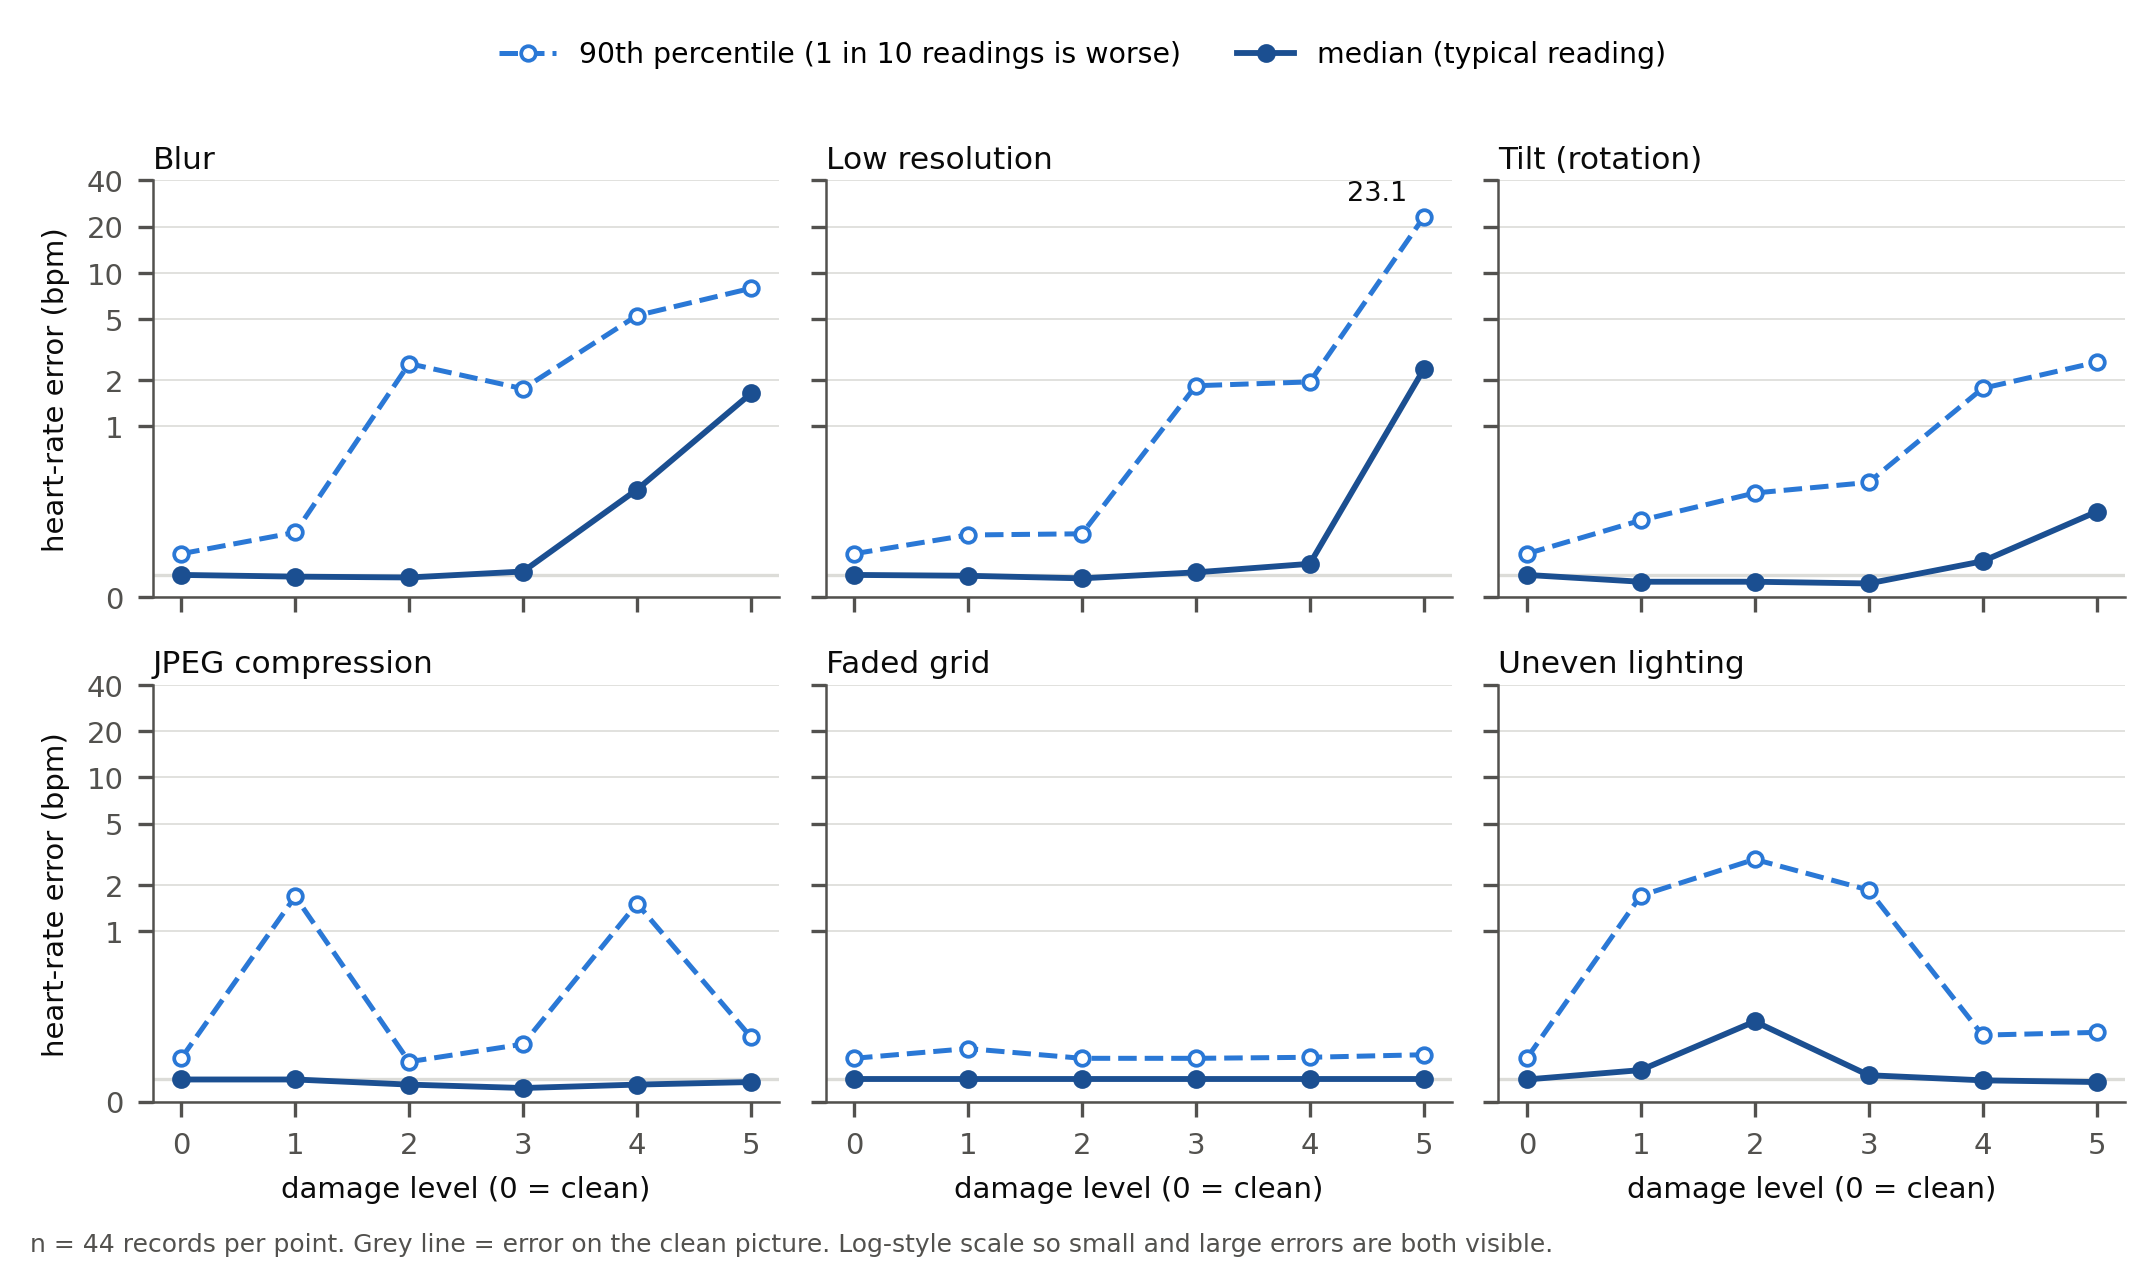
\includegraphics[width=\columnwidth]{figures/fig1_hr_error_by_damage.png}
\caption{Absolute heart-rate error (bpm, symlog scale) vs.\ degradation severity
(0~=~clean) for each of the six damage types, over the 44 reliable records. Solid
line: median; dashed line: 90th percentile. Grey line: median error on the clean
image. Only blur and resolution show a rising trend, and only at the highest
severities.}
\label{fig:fig1}
\end{figure}

\subsection{Patient-facing outcome: false reassurance and silent drops}

We classified each reading into the same slow/normal/fast bands used clinically
(\textless60, 60--100, \textgreater100~bpm) and compared the digitized band against
the ground-truth band, giving one of: correct, false alarm, \textbf{false
reassurance} (system reports normal when the truth is slow or fast), wrong-abnormal,
or silent drop (no reading produced). This is a heart-rate-only stand-in for the T3
``what the patient is told'' measure defined in Section~III-D; only 9 of the 44
reliable records have a truly abnormal ground-truth rate (6 slow, 3 fast), so this is
the size of the population that can produce a false reassurance at all -- the counts
below should be read as a pattern, not a stable rate.

On the clean images, all 44 reliable records were read correctly (0/44 errors).
Across the degraded images, 9 heart-rate readings were misclassified as normal when
the truth was abnormal; of these, 6 were \textbf{real} misreadings (digitized rate
more than 10~bpm from the true rate) and 3 were threshold artefacts, where a reading
a fraction of a beat from the 60 or 100~bpm boundary crossed the line without being a
clinically meaningful error (e.g., a true rate of 59.7~bpm read as 60.0~bpm). All 6
real false-reassurance events occurred at the \textbf{worst} severity level (level~5)
of the same two axes identified in Section~IV-C:

\begin{itemize}
\item \textbf{Low resolution, level~5:} 4 of the 9 at-risk records (44\%) were told
``normal'' when they were not, with readings off by 14--33~bpm.
\item \textbf{Blur, level~5:} 2 of the 9 at-risk records (22\%) were misread the same
way, off by roughly 15~bpm.
\item No false-reassurance events occurred at any other axis or at severity
levels~1--4 of blur or resolution.
\end{itemize}

Rotation produced a different failure: at its worst level, 4 of 44 reliable records
(9\%) yielded no reading at all (a silent drop) rather than a wrong one -- the
picture became unreadable before it became misleading. JPEG compression,
grid-contrast fade and brightness produced negligible false alarms and no false
reassurance at any tested level. Fig.~\ref{fig:fig2} summarizes both outcome types as
heatmaps across all six axes and five levels.

\begin{figure}[t]
\centering
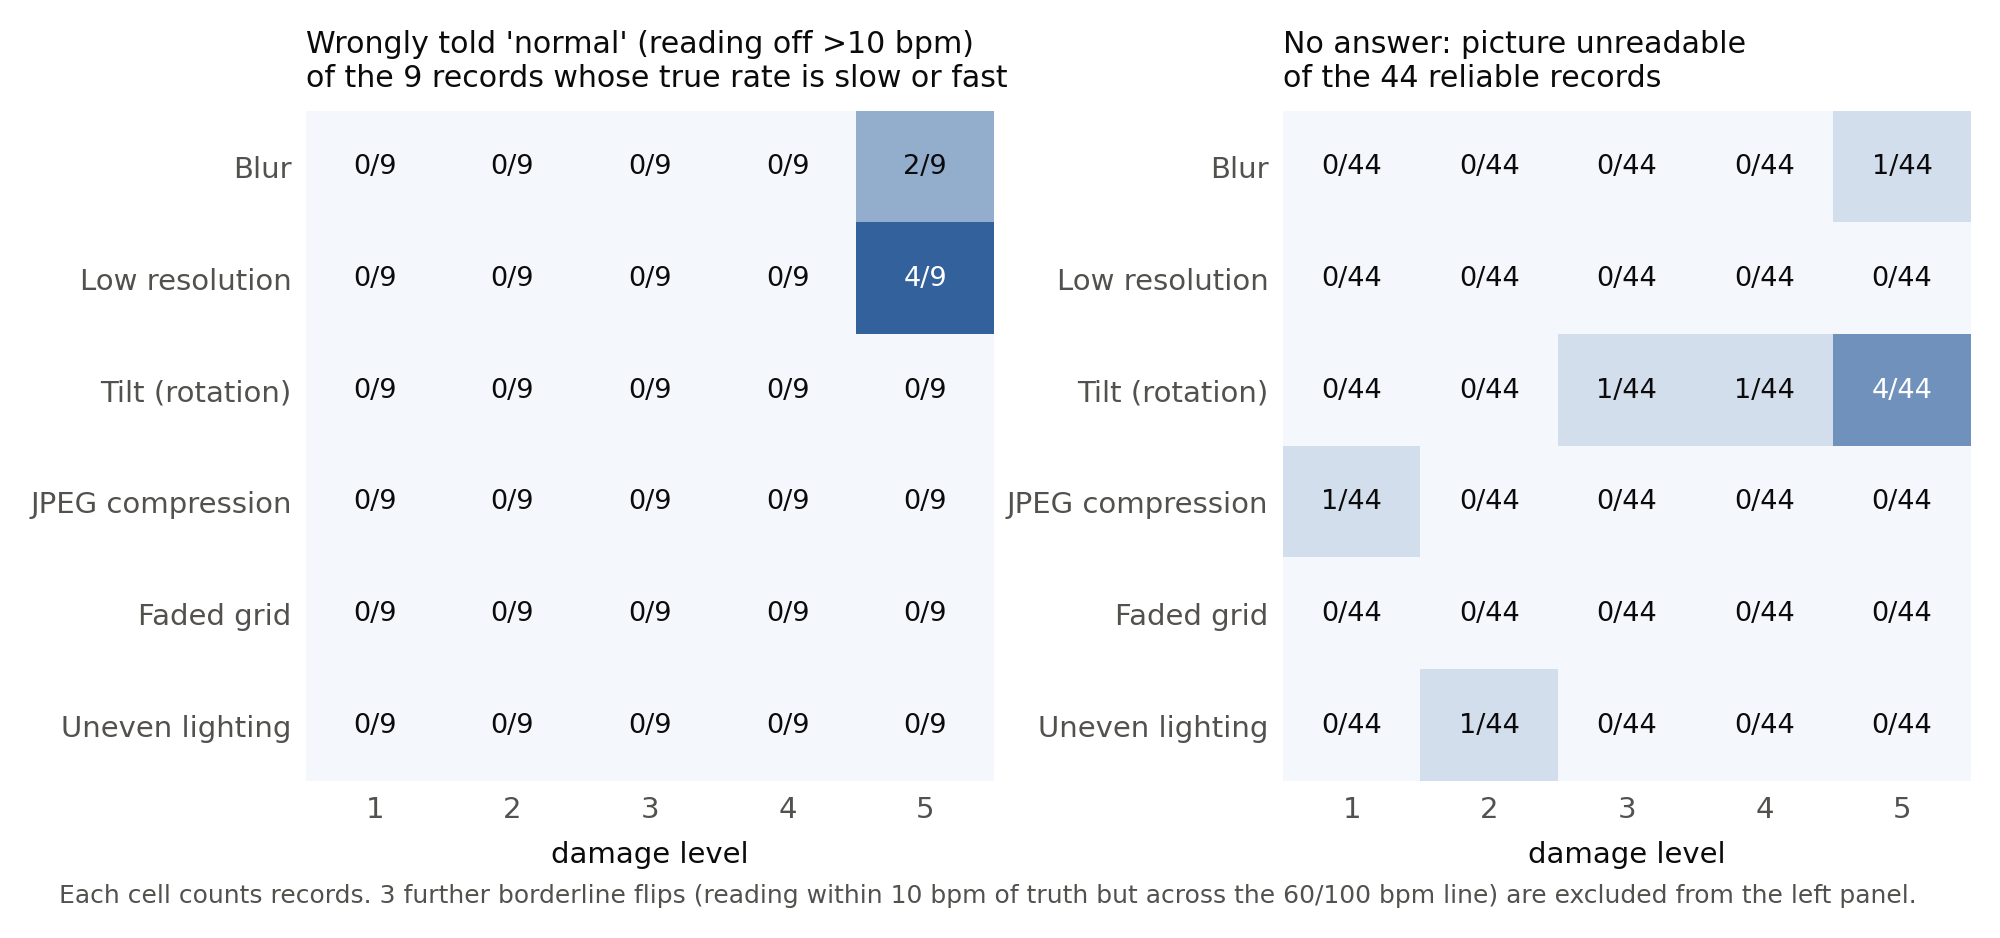
\includegraphics[width=\columnwidth]{figures/fig2_false_reassurance_and_silent_drops.png}
\caption{Left: of the 9 records whose true heart rate is slow or fast, how many were
misclassified as ``normal'' (reading off by $>$10~bpm) at each damage type $\times$
severity level. Right: of the 44 reliable records, how many produced no reading at
all, by damage type $\times$ severity level.}
\label{fig:fig2}
\end{figure}

\subsection{Summary of findings}

Within this sample and this pipeline: (1)~the system is reliable on clean images and
under mild-to-moderate degradation on every axis tested; (2)~it degrades gracefully
along four of six axes (rotation, JPEG, grid contrast, brightness), producing at
worst a ``no answer'' outcome rather than a wrong one; (3)~two axes -- heavy blur and
low resolution -- are qualitatively different: both produce a real, clinically
meaningful false-reassurance event, and both do so specifically at the most severe
level tested, with no warning at intermediate levels; (4)~roughly one record in eight
in this sample is unreliable for reasons independent of image quality, which is
itself an operational finding about the digitizer rather than about degradation.

\begin{figure}[t]
\centering
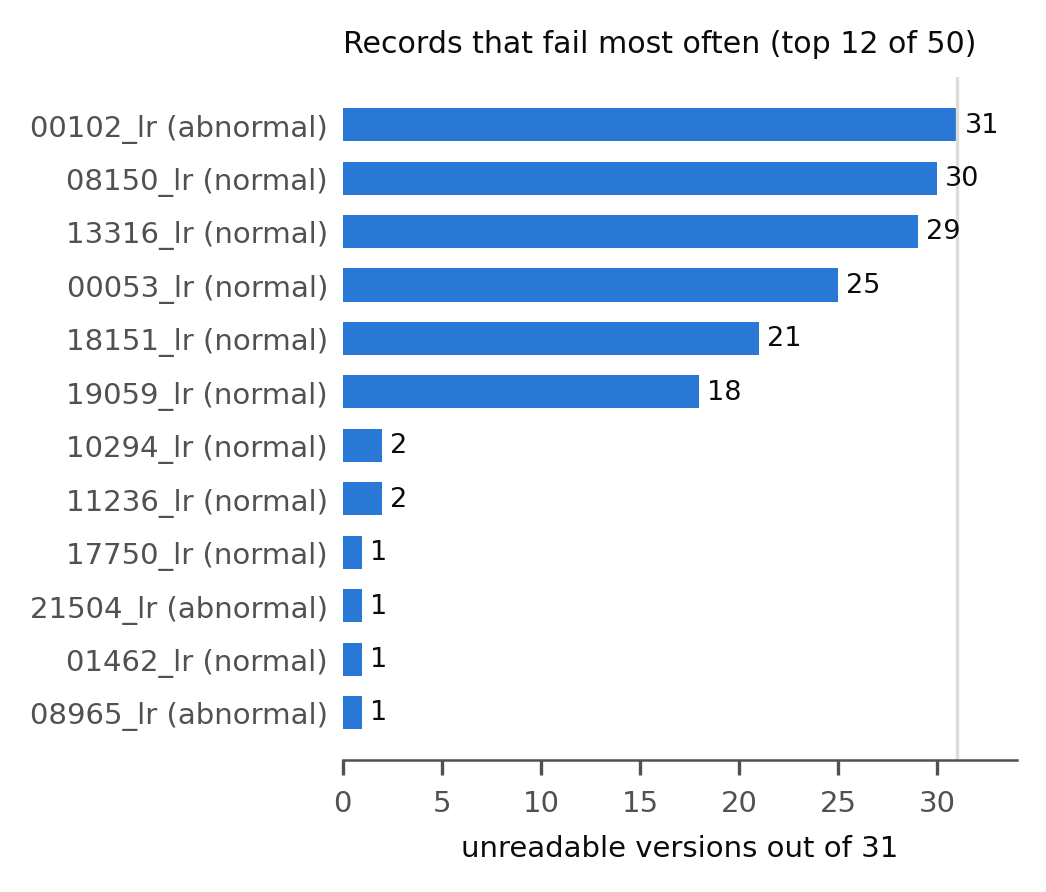
\includegraphics[width=\columnwidth]{figures/fig3_unreadable_records.png}
\caption{The 12 records (of 50) with the most unreadable versions out of 31
attempted; 6 fail in most versions, and 4 of those fail even on the clean image.}
\label{fig:fig3}
\end{figure}

\subsection{Interval-level (PR, QRS, QT, QTc) error confirms the pattern, with a
caveat}

A second sweep, run separately from the heart-rate results above (Section~VI notes
the reproducibility implication of this), retained the digitized signal to measure
PR, QRS, QT, and QTc (Section~III-E). Of the 50 records, 49 were reliably digitized
in this run -- a different reliability outcome than the 44/50 found for the original
heart-rate sweep (Section~IV-B); only one record (\texttt{15192\_lr}) failed badly (20
of 31 versions unreadable), and none of the four records that failed on their clean
image in the original run did so here. We report interval statistics over these 49
reliable records, not the earlier 44, since reliability was measured independently
for this data.

\textbf{Error magnitude confirms blur and resolution matter, on top of a real
baseline noise floor.} Even on the clean image, delineation-based interval
measurement disagrees between ground truth and digitized signal by a median of
20.2~ms (QTc), 25.3~ms (QRS), 16.9~ms (QT), and 13.5~ms (PR) -- far larger than heart
rate's 0.13~bpm clean-image error, because locating P/T-wave boundaries via wavelet
delineation is inherently more sensitive to small reconstruction differences than
counting R-peaks. On top of that baseline, the same two axes identified for heart
rate show a clear rising trend: median QTc error rises from 20.7~ms (blur level~1) to
101.8~ms (blur level~5), and from 21.7~ms to 77.2~ms across resolution levels~1--5.
The other four axes stay within the baseline band at every level (full table in
\texttt{results/v2\_intervals/summary\_intervals\_by\_axis\_level.csv}). This is
consistent with Section~IV-C at a different measurement, but it comes from the same
50 records and images, so it is a second view of the same data, not an independent
replication.

\textbf{QTc-based false reassurance: a smaller, less concentrated signal, reported
cautiously.} We classified each test's QTc against the sex-specific threshold
(Section~III-E) and compared to the same classification on ground truth, giving a
QTc analogue of false reassurance. A naive count found 39 such events -- but 32 of
these occurred on records whose \emph{own clean image} was already misclassified,
i.e.\ the $\sim$20~ms baseline noise alone was enough to push an already-borderline
record's QTc across the threshold, with no degradation involved. Counting these as
degradation-caused would be wrong, so we exclude them: a QTc false-reassurance event
counts as real only if (a) the same record's clean-image QTc was classified
correctly and (b) the digitized QTc differs from ground truth by more than 10~ms
(the same threshold-artefact discipline as Section~IV-D). This leaves \textbf{6 real
events}, spread thinly across blur (level~2), rotation (levels~4--5), resolution
(levels~1--2), and brightness (level~3), among 19 usable at-risk records (Wilson 95\%
CI per axis/level cell: 0.009--0.246, i.e.\ $n=1$ event in nearly every non-zero
cell). Unlike the heart-rate result -- concentrated at the single worst level of
exactly two axes, with 2/9 and 4/9 rates -- this QTc signal shows no comparable
concentration and is not, on this evidence, distinguishable from noise. We report it
as exploratory, not as a second confirmed false-reassurance channel.

\textbf{Robustness to the ground-truth sampling rate.} Because the ground truth above
came from 100~Hz records, we repeated the interval analysis with ground truth
recomputed from the same records at 500~Hz (digitized values unchanged). The
conclusions do not change: the clean-image median QTc error falls from 20.2 to
17.3~ms; blur and resolution still raise it steeply (to 90.8~ms at blur level~5 and
73.0~ms at resolution level~5) while the other four axes stay within a few
milliseconds of baseline; and the corrected QTc analysis again yields 6 real events
(26 apparent, 20 of them on records already misclassified on their own clean image),
scattered across blur, rotation, resolution, and brightness.

\section{Discussion}

\subsection{Two axes matter; four do not -- and the failure mode differs}

The central pattern in Section~IV is not that degradation is uniformly harmful, but
that it is sharply bimodal. Blur and low resolution are the only two of six tested
axes that produce a rising error trend (Section~IV-C) and the only two that produce a
real false-reassurance event (Section~IV-D) -- and in both cases only at the single
most severe level tested, with no detectable warning at intermediate severities. This
matters practically: a monitoring or quality-gating system cannot rely on a smooth
early-warning signal from these two axes. Error is effectively flat through level~4
and then jumps at level~5, so any usable quality threshold for blur or resolution
must sit clearly below that jump, not be tuned against a gradual curve.

The other four axes -- rotation, JPEG compression, grid-contrast fade, and
brightness/shadow -- behave differently in a way that is, if anything, reassuring for
system design. Rotation's worst failure mode is a \textbf{silent drop}: at its most
severe level, 4 of 44 reliable records (9\%) produced no reading at all rather than a
wrong one (Section~IV-C, IV-D). A system that returns nothing is trivially safer than
one that returns a confident wrong answer -- a silent drop is recoverable (the user
is asked to retake the photo) in a way a false reassurance is not. JPEG compression,
grid-contrast fade, and brightness/shadow produced neither a rising error trend nor a
meaningful rate of any bad outcome at any level tested, suggesting the digitizer's
extraction step is genuinely robust to these three particular failure modes within
the ranges we tested.

\emph{Why} blur and resolution might differ from the other four is worth stating as a
hypothesis, since we did not instrument the digitizer's internals to confirm it
directly: both axes destroy the same underlying signal -- the sharp edges of the
printed trace against the grid -- that grid detection and R-peak localization likely
depend on, whereas rotation is a global geometric transform the digitizer's layout
step may already correct for, and JPEG/contrast/brightness degrade appearance
without removing the trace's edges at the severities tested. We have not directly
verified this mechanism and present it as a hypothesis for future instrumentation,
not as a confirmed finding.

\subsection{Interval-level measurement is noisier than rate-based measurement, and
that itself matters}

Section~IV-F's baseline finding -- a $\sim$20~ms delineation disagreement between
ground truth and digitized signal on the \emph{undamaged} image, against essentially
none for heart rate -- is not a footnote; it is a finding about which patient-facing
measurements this kind of pipeline can currently support reliably. Heart rate, built
on R-peak counting, is robust enough that its clean-image error is negligible and its
false-reassurance signal is sharply concentrated and interpretable. PR/QRS/QT/QTc,
built on wavelet delineation of much smaller waveform features, start from a noise
floor large enough to flip an already-borderline record's classification before any
degradation is applied at all. Part of that floor is our own ground truth being
coarse (100~Hz), and part is intrinsic to delineating a reconstructed signal; we
measured the first but could not fully separate the two. A system that surfaces QTc-based safety statements to
a patient inherits this same noise floor, and our result suggests that doing so
responsibly would require either a more precise delineation method than we used here,
or an explicit uncertainty band around any reported interval -- not a bare number.
This is itself a concrete, practical argument for the uncertainty-qualified
explanation style proposed as this project's future no-reference quality work
(Section~VII): a system should not state a QTc value with the same confidence it
states a heart rate.

\subsection{Practical implication: where an upload-time quality gate should sit}

A natural extension of this work is deriving a minimum acceptable image-quality
threshold from exactly this kind of curve, to be enforced as an upload-time gate. The
results here suggest that gate does not need to be symmetric across all six axes: a
system could safely tolerate a moderately rotated, compressed, faded, or unevenly lit
photo, but should specifically flag or reject images that are heavily blurred or
captured at very low resolution -- the two conditions under which this study observed
real, clinically meaningful misclassification. This is a narrower and more targeted
claim than ``reject all poor quality images,'' and one this dataset, unusually,
supports directly.

\subsection{Engaging the abstention critique}

Jabbour et al.\ \cite{ref26} find that when a clinical AI system abstains,
clinicians' own error patterns shift rather than uniformly improve -- false positives
fall, false negatives rise. This is relevant to any future version of this system
that acts on the findings in Section~V-C by refusing to process a low-quality image:
a refusal is not automatically a safe outcome if it pushes a patient toward not
seeking care at all, rather than toward retaking the photo or consulting a clinician.
Our current results do not test this -- they measure whether the \emph{system's own
output} is wrong, not what a patient or clinician does downstream in response to a
wrong or withheld answer, which \cite{ref26}'s finding suggests is not a safe
assumption to skip. We treat this as an open question for any deployed version of the
quality gate proposed above, not as evidence against building one, but as a reason
its evaluation must eventually include what happens after the system declines to
answer, not only whether it declined correctly.

\subsection{Relation to the closest published work}

Section~II-B's cited quality-assessment literature asks whether a \emph{signal} is
good enough to analyze, typically reporting classification accuracy against a
human-labeled interpretable/non-interpretable ground truth \cite{ref12,ref13,ref14,ref15,ref16,ref17,ref18,ref19,ref20,ref21,ref22}.
Our results are not directly comparable to those accuracy figures, because we ask a
different question -- not ``is this readable'' in the abstract, but ``does the
number this system would report to a patient, given this specific image, match the
truth'' -- and report outcome rates at graded severities rather than a single
accuracy figure. We see this as an extension of the gap identified in Section~II:
carrying the quality question through to the sentence a patient reads, rather than
stopping at the signal.

\section{Limitations}

We state these plainly, as scope decisions and known weaknesses.

\begin{enumerate}
\item \textbf{Interval-level measurement has a real, documented noise floor, and the
QTc outcome result is exploratory.} Section~IV-F extends the outcome measure beyond
heart rate to PR/QRS/QT/QTc, but that measurement disagrees between ground truth and
digitized signal by a median of $\sim$20~ms even on undamaged images -- large enough
that a naive false-reassurance count was confounded by baseline noise until corrected
(Section~IV-F, Section~V-B). After correction, only 6 real QTc-based events remain
across 19 at-risk records, with no clear severity concentration; we do not claim this
as a second confirmed false-reassurance channel with the same strength as the
heart-rate result, only as a same-direction, less certain signal worth further work
with a more precise delineation method.
\item \textbf{The digitizer dependency is not version-pinned, and this measurably
mattered.} The sweep notebook clones the Open-ECG-Digitizer repository fresh each
session without pinning a commit. The interval-measurement sweep (Section~IV-F) was
run several days after the original heart-rate sweep, and none of the four records
that failed on their clean image in the original run failed in the later run; a
different single record failed instead. A test-by-test comparison of the two sweeps
shows that of the 1{,}367 tests that gave a heart rate in both, 99.3\% agree to within
0.15~bpm, and the six real false-reassurance events are the same six tests; only seven
records changed readability (six became readable, one became unreadable). The second
sweep is therefore a computational repeat of the same tests, not an independent
replication. We report both outcomes honestly rather than reconciling them, and flag
this as a concrete reproducibility gap: exact re-runs of
this study require pinning the digitizer to a specific commit, which this version of
the harness does not do.
\item \textbf{Sample size and its effect on the headline finding's precision.} The
study sample was reduced from a planned $\sim$500 stratified records to 50, for
compute-quota and deadline reasons decided before any result was observed
(Section~III-A). Of those 50, only 9 records have a truly abnormal ground-truth heart
rate, since a false-reassurance event can only be observed on an abnormal-truth
record. The false-reassurance counts in Section~IV-D (2/9, 4/9) should be read as a
pattern demonstrating \emph{that} the failure exists and roughly \emph{where} it
concentrates, not as a precise population rate; Wilson 95\% confidence intervals
computed over this sample are wide, consistent with $n=9$.
\item \textbf{A data-quality confound, reported and excluded rather than hidden.} Six
of the 50 sampled records (12\%) were unreadable by the digitizer in most of their 31
versions regardless of degradation, and 4 of those 6 failed even on the undamaged
clean image. We attribute this to per-record digitizer behavior unrelated to the
degradation under study and exclude these records from the degradation analysis
(Section~IV-B), reporting them separately. This is itself a finding about real-world
digitizer reliability, not only a methodological caveat, and we report it as such
rather than silently dropping the records.
\item \textbf{Simulated, not photographed, degradation.} All six degradation axes are
applied by post-processing a cleanly rendered image (OpenCV transforms), not
captured from an actual camera photographing a printed page. This isolates each axis
cleanly for controlled measurement, which real photographs rarely allow, but real
photos combine several of these conditions simultaneously (e.g., blur and uneven
lighting together) and may include failure modes this simulation does not reproduce,
such as physical creasing, glare, or partial occlusion -- several of which are
catalogued directly from real photographed ECGs in \cite{ref2,ref4} and would be a
natural extension of this degradation model.
\item \textbf{Single digitizer, single rendering tool, single lead.} All results use
one digitization tool (Open-ECG-Digitizer \cite{ref5}) and one rendering tool
(ECG-Image-Kit \cite{ref1}); the false-reassurance pattern reported here is a property
of this specific pipeline and may not generalize to other digitizers listed in
Section~II-A \cite{ref2,ref3,ref4,ref6,ref7,ref8,ref9,ref10,ref11} without re-running
the study against them. Measurements are also computed from lead~II only, matching
the pipeline's current scope, not the full 12-lead signal.
\item \textbf{Single-axis degradation.} Each of the six axes was varied independently
against an otherwise-clean image (Section~III-C), not in combination. Real
photographs plausibly combine multiple degradations at once (e.g., a tilted, dim
photo taken at a distance), and combined-axis effects may compound differently than
the single-axis curves in Section~IV-C would predict; this was out of scope for the
time available and is named here as future work, not silently assumed away.
\end{enumerate}

\section{Conclusion}

This paper measured, rather than assumed, how far degradation in a photographed
paper ECG propagates into what an automated system tells a patient. Using a
controlled, repeatable harness over a labeled sample of PTB-XL records, we found the
failure is not uniform across degradation types: heavy blur and very low resolution
are qualitatively different from rotation, JPEG compression, faded print, and uneven
lighting, both in whether they produce a rising error trend at all (Section~IV-C) and
in the kind of failure they cause when they do -- a wrong, falsely reassuring answer
for blur and resolution, versus a safer ``no answer'' for the others (Section~IV-D,
Section~V-A). This distinction is, to our knowledge, not previously reported for a
patient-facing ECG pipeline (Section~II), and it has a direct practical consequence:
an upload-time image-quality gate for a system like this does not need to reject
broadly degraded photos uniformly -- it needs to specifically catch heavy blur and
low resolution, the two conditions under which this study observed real harm.

The study also surfaced a finding independent of degradation itself: 6 of 50 sampled
records (12\%) were unreliable to digitize in most of their versions, including 4
that failed on the undamaged clean image. We report this as a real property of the
digitizer's reliability on this sample, not folded into the degradation curves, and
note it as a caution for anyone deploying a similar pipeline: image quality is not
the only source of failure worth measuring.

\textbf{Future work.} The most direct next steps, in order of value: (1)~pin the
digitizer to a fixed commit and re-run both the heart-rate and interval sweeps
together in one pass, resolving the reproducibility gap identified in Section~VI and
letting the two outcome measures be reported over the same reliable-record set;
(2)~improve interval delineation precision (or add an explicit per-measurement
uncertainty band) to shrink the $\sim$20~ms baseline noise floor identified in
Section~IV-F and V-B, which is the main obstacle to a QTc-based false-reassurance
result as strong as the heart-rate one; (3)~build and calibrate a no-reference
image-quality proxy, targeted specifically at the two axes shown here to matter, and
evaluate whether it predicts false-reassurance risk well enough to gate uploads
before digitization runs at all -- a first step on this is under way: five
image-level signals (blur, skew, effective resolution, contrast, and a JPEG-blockiness
measure) computable from a photograph alone were implemented and spike-tested on a
small set of demo pages, each moving monotonically with its targeted degradation
axis (Spearman $|\rho|$ 0.88--0.98). Computed for all 1,550 images of the present
study and compared against the measured errors above, four of the five correlate
with real QRS-duration error (blur $\rho=-0.306$, resolution $\rho=-0.285$, contrast
$\rho=-0.260$, blockiness $\rho=+0.085$, all $p<0.001$, $n=1509$; skew $\rho=-0.020$,
not significant), reproducing the same two axes shown above to matter. A
logistic-regression classifier on all five signals, fit and scored on the same 6
real QTc false-reassurance events (19 usable at-risk records, 589 tests), reached an
AUC of 0.785; that figure is optimistic and should not be read as a held-out result.
A stricter test holding out whole recordings (49 recordings, 1,519 tests; bad
reading = wrong by more than a fixed tolerance or unreadable) gave an AUC of 0.607
(95\% interval 0.49--0.82) for heart rate off by more than 5\,bpm, against 0.655 for
an oracle told the exact damage type and level; larger errors were better predicted
(heart rate $>$10\,bpm 0.825, QTc $>$60\,ms 0.767, QRS $>$100\,ms 0.736), but
leaving one damage type out of training gave AUCs of 0.32--0.37 for brightness, JPEG
and rotation, so the prototype does not yet generalise to unseen damage; (4)~extend the sample back toward the originally
planned $\sim$500 records to narrow the wide confidence intervals around both the
9-record heart-rate and 19-record QTc at-risk populations (Section~VI); (5)~test
combined-axis degradation, since real photographs plausibly combine several of these
conditions at once (Section~VI); and (6)~evaluate the abstention question raised in
Section~V-D directly -- what a patient or clinician does when the system declines to
answer, not only whether the decision to decline was correct.

More broadly, this work argues that ``does the digitizer work'' and ``is the final
patient-facing statement correct'' are different questions, and that safety claims
for systems of this kind should be evaluated against the second, not only the first.

\bibliographystyle{IEEEtran}
\bibliography{references}

\end{document}
